
\documentclass[11pt]{amsart}
\usepackage[usenames,dvipsnames,condensed]{xcolor}
%\usepackage[a4paper,right=.7in,left=.7in,top=.6in,bottom=.5in]{geometry}
\usepackage{fullpage}
\usepackage{amsmath}
\usepackage{mathtools}
\usepackage{amsthm}
\usepackage{amsfonts}
\usepackage[UKenglish]{babel}
\usepackage{graphicx}
\usepackage{cite}
\usepackage{multicol}
\usepackage{multirow}
\usepackage{afterpage}
\usepackage{sansmath}
\usepackage{marginnote}
\usepackage{verbatim}
%\usepackage{hyperref}

\usepackage{boxedminipage}
%\usepackage{titlesec}

\usepackage{hyperref}
\hypersetup{
    backref =       true,
    pagebackref  =  true,
    colorlinks =    true,
    linkcolor =     purple,
    anchorcolor =   [rgb]{0.0,0.0,0.0},
    citecolor =     [rgb]{0.0,0.0,0.0},
    filecolor =     [rgb]{0.0,0.0,0.0},
    urlcolor =      [rgb]{0.0,0.0,0.0},
    pdftitle=       {Title},
    pdfsubject=     {Title},
    pdfauthor=      {K. Sasaki}
}
 
%\reversemarginpar

\setcounter{tocdepth}{4}
\setcounter{secnumdepth}{4}

%\titleformat{\paragraph}
%{\normalfont\normalsize\bfseries}{\theparagraph}{1em}{}
%\titlespacing*{\paragraph}
%{0pt}{3.25ex plus 1ex minus .2ex}{1.5ex plus .2ex}



%\usepackage{fancyhdr}
%\pagestyle{fancy}
%\lhead{Predoc/EMBO CBB courses, script}
%\rhead{Karin Sasaki}

%------------------------------------------------------------------------------------------------------------%


\begin{document}
%\twocolumn
\title{Fundamentals of MATLAB}
\author{Karin Sasaki (EMBL Centre for Biological Modelling)}

\maketitle

\tableofcontents

\clearpage
\section{Introduction to MATLAB}

\subsection{MATLAB windows, variables and output}

\

MATLAB (Matrix Laboratory) is a language for technical computing. It is based on matrix (array) operations; It integrates computation, visualisation, and programming and is a numerical software.

\subsubsection{MATLAB Tabs}
There are various tabs that can be used to carry out tasks, interactively (see figure \ref{figA}). These include the Home tab (where you can create new scripts, open previous ones, set preferences, etc) and the Apps tab (add ons to MATLAB to enable other functionalities, e.g. curve fitting, image processing, statistical analysis, optimisation, etc). Other tabs have functionalities relevant to other tasks.

\begin{figure}[h]
\centering
\caption{Tabs (in red) and Windows (in purple).}
\label{figA}
	 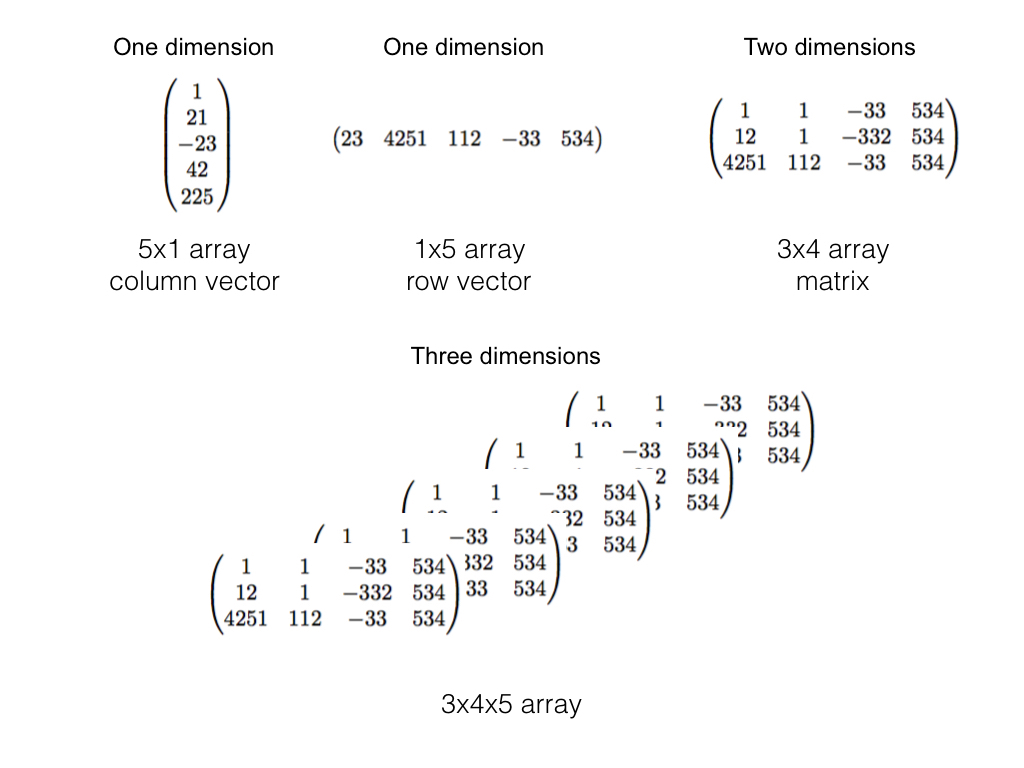
\includegraphics[width=1\textwidth]{figA}
\end{figure}

\subsubsection{MATLAB Windows}
(See figure \ref{figA})

\

{\bf Command Window: }The command window is suited to perform a small set of operations or for testing purposes. 
e.g. type the following in the command window and see what happens:

\

\color{blue}
\begin{verbatim}
2 + 2
\end{verbatim}
\color{black}
or
\color{blue}
\begin{verbatim}
% display i = from 1 to 10
for i = 1:10 
	i
end
\end{verbatim}
\color{black}

\

{\bf Note:} The symbol $\%$ indicates to MATLAB that it can ignore whatever is on the same line and follows the $\%$, so you can use this to make comments on commands, to clarify to others (and remind yourself) of what you are intending to do.

\

{\bf Variables:} Variables are characters that represent a value. To initialize a variable with a value, the operation = is used. 
e.g.

\

\color{blue}
\begin{verbatim}
my_variable = 2 + 2
\end{verbatim}
\color{black}

\

This variable will have the value of 4. So whenever you type \verb+my_variable+ on the command window, it will output the value 4. 

\

Variable names must start with a letter and can contain numbers and other symbols. Almost any word can be assigned to a value, with a few exceptions. To check which words cannot be used as variable names, type \verb+iskeyword+ in the Command Window: 

\

\color{blue}
\begin{verbatim}
iskeyword % none of these words can be used to name variables.
\end{verbatim}
\color{black}

\

{\bf Suppress output on the Command Window:} MATLAB prints out the result of whatever operations you perform on the Command Window. If you want to avoid this, use a semicolon at the end of the line.

\

\color{blue}
\begin{verbatim}
my_vec = [1 2 3 4 5 6 7 8 9 10];
my_sum = sum(my_vec);
\end{verbatim}
\color{black}

\

{\bf Workspace Window:} This window shows the variables you have defined, their values and information about them. (In case you cannot see the window, type \verb+workspace+ on the Command Window.) 

\

{\bf Command History Window:} This window display a log of statements that you have ran on the current and previous MATLAB sessions. (In case you cannot see the window, type  \verb+commandhistory+ on the Command Window.)

\

{\bf Editor Window:} To automatically analyse data or images, or simulate models, it is recommended to write {\it script} or {\it function files}. The Editor Window facilitates this, by providing a means of collecting all necessary commands for a specific task on to one file. We will learn more about this below. (In case you cannot see the window, type  \verb+edit filename+ on the Command Window, where the filename is the name of the file you want to creadte/edit. It will be saved on the current folder, shown on the Current Folder Window (see below).)

\

{\bf Current Folder Window:} This window lets you navigate folders. It shows the current working folder, from where you can load variables and files and on which any changes are saved. (To open this window, type  \verb+filebrowser+ on the Command Window.)

\

{\bf Variables Window:} Displays the values of the variables that are on the Workspace.

\

{\bf Figures Window:} Displays figures. It opens when you plot a figure.

\

\subsubsection{Saving your work}

\

\

{\bf Save the Command Window:} It might be helpful to save the commands you use on the Command Window and the output (remember that the Command History records only the commands). To do so, create a .txt file by typing the following on the Command Window:

\

\color{blue}
\begin{verbatim}
diary thursday_20th % today is the name of the .txt file where the commands and output after
 this line will be saved.

% Type some commands ...

diary off % stops recording 
\end{verbatim}
\color{black}

\

As a measure of safety, make sure that you save your work every now and then, by typing \verb+diary off diary on+. Commands carry on being saved at the bottom of the text file.

\


{\bf Save the Workspace (the variables you are working with):} You might want to reuse the variables you are currently working with, sometime in the future, so it is a good idea to save them. To do that type the following on the Command Window (where the filename is chosen by you)

\

\color{blue}
\begin{verbatim}
save filename % this saves the variables to a file with .mat extension
load filename % this loads the variables to the Workspace
\end{verbatim}
\color{black}

\

Clear the Command Window: type on the command window 

\

\color{blue}
\begin{verbatim}
clc
\end{verbatim}
\color{black}

\

Clear the Workspace: type on the Command Window:
\

\color{blue}
\begin{verbatim}
clear
\end{verbatim}
\color{black}

\

Be careful not to confuse the two!

\

Now try exercise 2.1.

\subsection{Arrays and operations on arrays}

\

MATLAB was originally written to ease dealing with tools of linear algebra - vectors and matrices (here referred to as {\it arrays}).

\

An {\bf array} is a multi dimensional grid of data. Tables in Microsoft Excel can be thought of as arrays with dimensions $r \times c \times p$ corresponding to $r$ rows $c$ columns and $p$ pages. In MATLAB it is similar, but using arrays is facilitated. Figure \ref{figB} illustrates arrays of different dimensions. 

\

\begin{figure}[h]
\centering
\caption{Arrays with different dimensions.}
\label{figB}
	 \includegraphics[width=1\textwidth]{figB}
	 
	 $r \times c \times p$ array
	 
 	 \includegraphics[width=.5\textwidth]{fig_arrays}
\end{figure}

\

Arrays are fundamental to MATLAB, as all data is stored in this format. It can also be useful to have data in this format; for example, it can make sense to store images as arrays (figure \ref{figC}) and as we will see, they are ideal to store stoichiometric information of a set of chemical reactions (figure \ref{figD}).

\

\begin{figure}[h]
\centering
\caption{An image is a set of data that is real-valued, ordered and represents color and intensity. Arrays are ideal for storing this type of information.}
\label{figC}
	 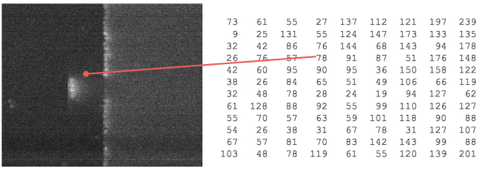
\includegraphics[width=1\textwidth]{figC}
\end{figure}

\

\begin{figure}[h]
\centering
\caption{Stoichiometric information of a simple enzymatic reaction stored in an array.}
\label{figD}
	 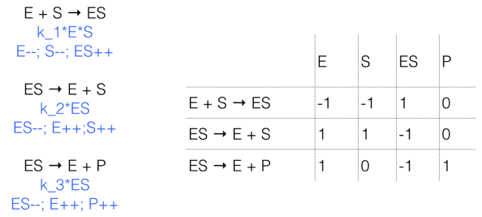
\includegraphics[width=0.7\textwidth]{figD}
\end{figure}

\

{\bf Create arrays:} by specifying values using squared brackets, commas, spaces and semicolons
e.g.

\

\color{blue}
\begin{verbatim}
a = [1 2 3 4 5 6 7 8 9] % a row vector, also called a 1x9 array
b = [5; 6; 3; -1; 6; 9; 2; 5; 5] % a column vector, also called a 9x1 array
A = [1 2 3 4 -1 -2 -3 -4;5 6 7 8 -5 -6 -7 -8] % a 2x8 matrix or array 

% Equally spaced arrays
c1 = 1:10 % with a step of 1
c2 = 1:2:10 % increasing with a step of 2
c3 = 10:-2:1 % decreasing with a step of 2
\end{verbatim}
\color{black}

\

{\bf In-built array functions:} MATLAB has in-built tools (called functions) for creating arrays. Note the use - call the function name, provide input to the functions inside round brackets and possibly allocate the result to a new variable.

\

\color{blue}
\begin{verbatim}
d = linspace(1,20,7) % linearly spaced row vector, between 1 and 20, with 7 entries
B = ones(3,3) % a 3x3 array with all entries 1
C = zeros(5,2) % a 5x2 array with all entries 0
D = eye(4,4) % 4x4 identity matrix, i.e. with 0's everywhere, except on the diagonal, 
which are 1's
E = rand(1,10) % 1x10 array with entries in [0,1] randomly chosen
e = randi(2,10,10) % 10x10 array with entries either 1 or 2, randomly chosen 
\end{verbatim}
\color{black}

\

{\bf Indexing:} Access and change individual entries in arrays, by indicating the name of the array and the rows and columns inside round brackets. Note the use of `:'  to create a range:

\

\color{blue}
\begin{verbatim}
% acess specific entries of arrays
A(1,2) % is the element of A in col 1 row 2
A(1,1:3) % are the elements of A in row 1, cols 1 through 3 
A(1,:) % is all the entries in row 1
A(1,2:end-1) % all the entries in row 1 except the first and last, defined using 
	 							    % the |end| keyword
 
% Assign values to specific entries in array: 
A(1, 2:end-1) = 10 % all entries of row 1 in A, except the first and last, 
                   % are equal to 10

% Delete one or more rows of an array: 
A(1:2, :) = [] % assign rows 1 and 2 of A to the empty array
\end{verbatim}
\color{black}

\

{\bf Linear indexing:} all arrays can also be thought of as a one column array, from top to bottom, left to right, so 

\

\color{blue}
\begin{verbatim}
A(2) % accesses element 2 top to bottom, left to right
A(:) % displays A as a column vector.
\end{verbatim}
\color{black}

\

{\bf Logical indexing:} You can use the logical operators $>,\ >=,\ <,\ <=,\ ==,\ |,\ \&$ (greater than, greater than or equal to, less than, less than or equal to, equal, or, and) to test entries in arrays, as follows:

\

\color{blue}
\begin{verbatim}
a<0.5 % gives the entry values of the elements of a that are less than 0.5.

a(a<0.5)=-1 % assigns the value -1 to all entries a that are < 0.5.

find(a) % gives the the linear indexes of a that are non-zero (see the help)

% Extract useful information:
[r,c] = find(a) % gives the row and column index of the non-zero elements of a.
 
A_length = length(A) % displays the length of A and assigns it to variable
                     % A_length
[Am, An] = size(A) % displays the dimensions of A and assigns them to Am
                   % and An, respectively
\end{verbatim}
\color{black}

\

{\bf Indexing with arrays:} 

You can also index arrays with arrays, as follows:

\

\color{blue}
\begin{verbatim}

% define an array 
F = rand(5,5);   

output:
F =

    0.9797    0.5949    0.1174    0.0855    0.7303
    0.4389    0.2622    0.2967    0.2625    0.4886
    0.1111    0.6028    0.3188    0.8010    0.5785
    0.2581    0.7112    0.4242    0.0292    0.2373
    0.4087    0.2217    0.5079    0.9289    0.4588

% find elements in array that are >=0.1. This gives an array of the same 
dimensions as f, with 1's where the logical statement evaluates as true and 0 elsewhere.
f = (F >= 0.1)

output:
f =

     1     1     1     0     1
     1     1     1     1     1
     1     1     1     1     1
     1     1     1     0     1
     1     1     1     1     1

% change the values that are >=0.1 to 0, by indexing F with f
F(f) = 0;

output:
F =

         0         0         0    0.0855         0
         0         0         0         0         0
         0         0         0         0         0
         0         0         0    0.0292         0
         0         0         0         0         0
\end{verbatim}
\color{black}

\


{\bf Arithmetic with Arrays:} Addition, multiplication, substraction, division, powers.

\

\color{blue}
\begin{verbatim}
a*b % standard array multiplication (see figure 5A)
a.*b % multiplication element by element (see figure 5b)
a.^2  % raise each element of a to the power of 2
a./2 % divide each element of a by 2
\end{verbatim}
\color{black}

\

\begin{figure}[h]
\centering
\caption{(A). Standard array multiplication. (B). Element-by-element array multiplication.}
\label{figE}
	 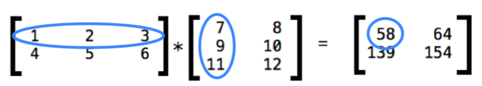
\includegraphics[width=0.7\textwidth]{figE}
	 
	 (A) $1*7 + 2*9 + 3*11 = 58$
	
	\
	
	 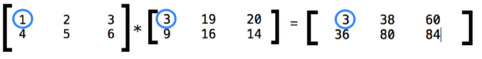
\includegraphics[width=0.8\textwidth]{figF}	 
	 
	 (B) $1*3 = 3$
\end{figure}

\

{\bf Array manipulation:} Array can be manupulated in many ways. Below are two examples. Other functions include \verb+fliplr, flipud, repmat, reshape, sort+.

\

\color{blue}
\begin{verbatim}
large_A = [A, A, A]; % Concatenates array A on the row direction - i.e. places them 
next to each other.

B = A' % the transpose of A, it exchanges the rows and the columns
\end{verbatim}
\color{black}



\subsection{Help and Documentation}

\

You have already used many of the tools (functions) MATLAB has on offer. You might want to read more about how those functions are used, and you should! To do so, you can type in the Command Window:

\

\color{blue}
\begin{verbatim}
help functionname
\end{verbatim}
\color{black}

\

You can also check the $f_x$ symbol on the Command Window 
or google the MATLAB documentation and search the name of the function there.

\

Now try exercise 2.2.

\subsection{Data types}

\

By now, you already understand what variables are, how to create them (section 1.1) and where and how you can look up information about them (Workspace Window). Now we will learn to understand that information:

\

Data may come in many different forms, for example, numerical (e.g. intensity values of a FRET imaging experiment), textual (e.g. names of proteins) or more complex (e.g. both of the above). In theory, you could have all your data as an array, but in practice, it may make more sense to make use some of the other variable types that MATLAB has, such as {\it cells} and {\it structures} (amongst others). The {\it class} or {\it type} of the variable describes the characteristics of the variable and the manipulations that can be applied to it. 

\

{\bf Numerical variables (default data type):} Arrays that have integer and floating point data
e.g. 

\

\color{blue}
\begin{verbatim}
a = 1.5; 
A = randi(10,10);
\end{verbatim}
\color{black}

\

{\bf Logical or boolean variables:} Arrays that have true or false data, displayed by 1 or 0 respectively. They are created by 
relational operators, as seen above (see also in Documentation, Logical Operators, for more details).
e.g.

\

\color{blue}
\begin{verbatim}
B = a > 1;  
C = isempty(A);
\end{verbatim}
\color{black}

\

{\bf Textual/string variables:} arrays with strings and characters, specified using ' ':

\

\color{blue}
\begin{verbatim}
A = 'John'
 \end{verbatim}
\color{black}

\
 
{\bf Structure variables:} A structure array is a data class that groups related data using containers called {\bf fields}. Each field can contain any type of data. Let's create a  {\it structure variable}, called \verb+fiber+, which we will use to store locational information on  dummy microtubules that make up a mitotic spindle:   \verb+fiber+ has two {\it fields} called  \verb+id+ and  \verb+pts+ which contain information about the fiber id and the $(x,y,z)$-coordinates of the points that make up a fiber, respectively. 

\color{blue}
\begin{verbatim}
% initialise a struture variable
fibers(10).id = []; % this defines a structure variable fiber with field id and 10 entries. 
                    %For the moment, every entry is the empty array.
fibers(10).pts = []; % this adds another field, pts, to the structure variable fibers. 
                     %Every entry is the empty array.
                     
% replace entries with specific data
fibers(1).id = 1;
fibers(2).id = 2;
.
.
.
fibers(10).id = 10;
fibers(1).pts = randi(100,3,3);
.
.
.
fibers(10).pts = randi(100,3,3);
\end{verbatim}
\color{black}

\begin{figure}[h]
\centering
\caption{Structure variable.}
\label{FigG}
	 \includegraphics[width=1\textwidth]{figG}
\end{figure}

\

When you open the variable \verb+fiber+ in the Variables Window, it should look as in figure \ref{FigG}.

\

To access data in a structure variable, use the row number and the field name: \verb+structName(i).fieldName+. For example, if you want the coordinates of fiber 2, type \verb+fiber2_pts = fiber(2).pts+.

\

%\

%\color{blue}
%\begin{verbatim}
%iFF708.rxn_Name(5) % MATLAB outputs the name of the 5th reaction.
%\end{verbatim}
%\color{black}

\
 
{\bf Cell Variables:} Arrays that can contain data of varying types and sizes - compare with  standard arrays and structure arrays. To define:

\

\color{blue}
\begin{verbatim}
myCell = {1, 2, 3; 'text', rand(5,10,2), {11; 22; 33}}
% This cell variable has 6 entries: the first three are of numerical type, 
the 4th is of character type, the 5th is again numerical and the 6th is a cell 
(a cell inside a cell).

myCell2 = cell(2,3) % this is an empty cell with 2 rows and 3 columns
\end{verbatim}
\color{black}

\    
          
You can see the class/type of your variables on the Workspace Window or by typing \verb+whos+ on the Command Window. For further information on these and other variables, see the MATLAB documentation.

\

Now try exercise 2.3.

\subsection{MATLAB Functions (tools) to manipulate arrays}

\

To manipulate arrays, you have already used MATLAB functions such as \verb+find+, \verb+size+ and \verb+cat+. Here are some of the general rules when it comes to using these, along with some examples. Remember that you can look these functions up on the MATLAB Documentation. 

\

To use functions, enclose inputs to functions in round brackets:

\

\color{blue}
\begin{verbatim}
max(A)
\end{verbatim}
\color{black}

\

Separate multiple inputs with commas:  

\

\color{blue}
\begin{verbatim}
max(A,B)
 \end{verbatim}
\color{black}

\

Store output from a function by assigning it to a variable: 

\

\color{blue}
\begin{verbatim}
maxA = max(A)
 \end{verbatim}
\color{black}

\

Enclose multiple outputs in square brackets: 

\

\color{blue}
\begin{verbatim}
[maxA, location] = max(A)
 \end{verbatim}
\color{black}

\

Basic in-built array functions include: \begin{verbatim}*, /, +, -, /*, ./, .^, log, sin, sum, mean, var, std, max, min, find...\end{verbatim}
 
 \
 
To stop execution: ctrl+C

\

Now try exercise 2.4.

\subsection{M-files - scripts}

\

Instead of running commands on the Command Window one by one, you can collect all of them into one file. This is done on the Editor Window. To open the window, type 

\

\color{blue}
\begin{verbatim}
edit filename
\end{verbatim}
\color{black}

\

and replace filename with the name you want to give the file. This will create a new file in your current folder, with extension .m

\


Let's calculate and plot the sine wave. Type the commands below into a new file on the Editor Window, save the file and run it by simply calling the name of the file on the Command Window.

\

\color{blue}
\begin{verbatim}
x = 0:1:6*pi;           % Define the range for x.
y = sin(x);             % Calculate y = sin(x).
plot(x,y)               % Plot y = sin(x).
 
% modify plot properties
title('Sine Wave')
xlabel('x')
ylabel('y = sin(x)')
\end{verbatim}
\color{black}

\

Now try exercise 2.5.


\clearpage
\section{Introduction to MATLAB - Exercises}

\subsection{MATLAB Windows, variables and output}
\begin{enumerate}
\item If you haven't done so already, start a MATLAB session and navigate to a directory of your choice.
\item Create a diary to save the Command Window.
\item Using the command window:
	\begin{enumerate}
	\item Compute the following quantities and assign them to variables.
	\item Suppress the output of some of them.
		\begin{enumerate}
		\item 1111-345
		\item cos(0.1)
		\item log(cos(0.1))
		\end{enumerate}
	\end{enumerate}
\item Save your Workspace and finish saving the Command Window to your diary.
\item Clear the Command Window but not the Workspace.
\end{enumerate}

\subsection{Arrays and operations on arrays}
\begin{enumerate}
\item Create a $3 \times 3$ random integer array A and two $3 \times 1$ integer vectors \verb+a+ and \verb+b+. (Hint: type \verb+help randi+ in the Command Window).
\item Multiply \verb+a+ by the scalar 5 and name this new vector c.
\item Compute \verb+a'*b+, \verb+a*b'+ and the element-wise product of \verb+a+ and \verb+b+. What do you get?  Why? (Hint: \verb+help transpose+ is helpful here).
\item What do you get for \verb+A(1,2), A(:, 3), A(1:2, 1:2)+? 
\item Replace the second column of \verb+A+ with \verb+b+ (Hint: the indexing section above is helpful).
\item Extract the following from \verb+A+: 
	\begin{enumerate}
	\item row 2, column 1
	\item row 3, all columns
	\item rows 2,3 columns 2,3 
	\end{enumerate}
\item Compute the (standard array) product of \verb+A+ and \verb+b+. What do you get? Can you do the element-wise product? Why/why not?
\item Concatenate \verb+b+ with itself 3 times to get a $3 \times 3$ array \verb+B+.
\item Multiply \verb+A+ and \verb+B+ element-wise and assign the result to a new variable \verb+C+.
\item Use the MATLAB function \verb+size+ to save the dimensions of \verb+C+ in \verb+rC+ and \verb+cC+. If necessary, use the MATLAB help by typing \verb+help size+ in the Command Window.
\item Use help to get information about \verb+length+ - how does it differ from \verb+size+?
\item Delete the first row of \verb+C+.
\item What are the dimensions of this new array?
\item Find the elements of \verb+C+ that are less than 5, both in linear indexing and row and column indexing. (Hint: Use the command \verb+find+.)
\end{enumerate}

\subsection{Data types}
\begin{enumerate}
\item Create a string (or char) variable \verb+name+ with your name.
\item Create a string (or char) variable \verb+sentence+ with a statement that makes sense when you put it together with the string variable \verb+name+. 
\item Concatenate the variables name and sentence into \verb+new_sentence+. Remember that you can use squared brackets of the function \verb+cat+.
\item Generate a random integer matrix \verb+K+ and a zeros matrix \verb+L+, both of the same dimensions. Create a logical variable \verb+M+ to the relational operation \verb+K == L+.
\item Create a structure called molecules with three fields: name, weight and test, and two entries for each field (make up the data).
\item Use the Workspace and the commands \verb+who+ and \verb+whos+ to get information about the variables that you currently have and make sure you understand it. 
\item Use the  Variables Window to examine the variables you have created. To do this, simply double click on the variable you want to inspect.
\end{enumerate}

\subsection{MATLAB Functions to manipulate arrays}
\begin{enumerate}
\item Create a $24 \times 3$ matrix \verb+Q+.You can think of \verb+Q+ as representing some biological data.
\item Calculate minimum, maximum, mean and standard deviation of each column of \verb+Q+. Use help for find out about the functions \verb+min+, \verb+max+, \verb+mean+ and \verb+std+.
\item Get the row numbers where the maximum data values occur in each data column. Remember to specify output parameters to return these. 
\item Substract the mean from each column of the matrix. (Hint: the \verb+repmat+ function is helpful here).
\item Save your current Workspace.
\end{enumerate}

\subsection{Script files}
\begin{enumerate}
\item Write a script file that creates a random vector with 1,000 elements, computes the sum of the squared elements of this vector (see \verb+help sum+) and outputs the resulting sum.
\item Use \verb+tic toc+ to see how long it takes the computer to do this takes (see \verb+help tic+)
\end{enumerate}





\clearpage
\section{Introduction to programming}

\subsection{M-files - functions}

\

You can write your own functions, which would work similar to the the MATLAB functions that you have used above (e.g. \verb+size, length+, etc). That is, your functions should  take input values, which are variables saved on the Workspace, and they will give you output, which ideally, you would assign to other variables. Like scripts, functions are also written on the Editor Window, and they also have a .m extension. But they differ from script files. (We will discuss the differences later.)

\

The example below shows the structure of a function file (type these commands onto a new file on the editor window and save as \verb+my_factorial.m+):


\

\color{blue}
\begin{verbatim}        
function f = my_factorial(n)
%
% f = my_factorial(n) is a function that calculates the factorial of 
% any integer. It takes in one input, which must be positive integer 
% value and outputs the factorial of that input, i.e. $(n*(n-1)*...*1)$.
%
 
f = prod(1:n);
\end{verbatim}
\color{black}

\


Line 1 indicates to MATLAB that this is a function file, that it has an output (\verb+f+), the name of the function (\verb+my_factorial+) and that it requires an input (\verb+n+). Lines 2-6 are comments that explain what the function does and how to use it. Line 7 is blank and line 8 has the commands that define the output, given the input. In summary, the parts of a function are the definition of the script as a function, a name, formal parameters (input/output (return)), specification and body.

\

Once you have saved the function to an .m file, type in the Command Window

\

\color{blue}
\begin{verbatim}
help my_factorial
\end{verbatim}
\color{black}

\

The comments that explain the function show up, just like for any other MATLAB function. Now try using this function like any other MATLAB function, e.g. as follows:

\

\color{blue}
\begin{verbatim}
f10 = my_factorial(10)
\end{verbatim}
\color{black}

\

This should output \verb+f10 = 3628800+.

\

Function files can have as many inputs and outputs as you like. Here is how:

\
 
If your function accepts more than one input: 
\color{blue}
\begin{verbatim}
function V = cell_volume(x, y, z) 
\end{verbatim}
\color{black}

\

 
If more than one output is needed: 
\color{blue}
\begin{verbatim}
function [pull drag] = motor_movement(x)
 \end{verbatim}
\color{black}

\

If no output is needed: 
\color{blue}
\begin{verbatim}
function my_fun(x) 
\end{verbatim}
\color{black}

\

or 

\

\color{blue}
\begin{verbatim}
function [] = my_fun(x)
 \end{verbatim}
\color{black}

\

{\bf Note of precaution:} Remember that you need to make sure that your function works on arrays with dimensions that make sense for what you intend to do. So do not forget taking care of $.*$, sizes, etc. Note that \verb+my_factorial+ currently only works on arrays with dimensions 1x1.
 
 \
 
{\bf Note:} Remember to make comments and add a help section to all your functions! This looks like unnecessary work, but when you start writing very long programs, it will save you a lot of time.

\

Now try exercise 4.1.

\subsection{Scripts vs functions}

\

See table \ref{tableA}.

\begin{table}[h!]
\caption{}
\label{tableA}
\begin{tabular}{|c|p{7cm}|p{7cm}|}
\hline
 & {\bf Scripts} & {\bf Functions}\\\hline
$=$ & Contain MATLAB code. & Contain MATLAB code.\\\hline
$=$ & Stored in files with a .m extension. & Stored in files with a .m extension.\\\hline
$\neq$ & Scripts execute a series of MATLAB statements; `input' must be defined in script or the Workspace; outputs all variables calculated. & Functions accept input arguments defined in the workspace only, execute a series of MATLAB statements and produce only specific output. \\\hline
$\neq$ & Not easily used for modulation of your programs. & Easily used for modulation of your programs.\\\hline
\end{tabular}
\end{table}

\

For example:

\

write a *script* called \verb+triangle_area+ with the commands below and run it by calling the name of the file on the Command Line

\

\color{blue}
\begin{verbatim}
b = 5;
h = 3;
a = 0.5*(b.* h)
 \end{verbatim}
\color{black}

\

vs 

\

make a *function* 

\

\color{blue}
\begin{verbatim}
function a = triangle_area(b,h)
%
% Description:
% Calculates the area of a triangle
%
% Input:
% |b| is the base
% |h| is the heigh
% 
% Output:
% |a| the are of the triangle
%
 
% Area of triangle
a = 0.5*(b.* h);
 \end{verbatim}
\color{black}

\


Now call in the Command Window as follows

\

\color{blue}
\begin{verbatim}
a1 = triangle_area(1,5)
a2 = triangle_area(2,10)
a3 = triangle_area(3,6)
\end{verbatim}
\color{black}

\

{\bf Note:} Remember to make functions and scripts array-friendly - if you expect to make calculations with arrays, make sure you are doing the correct arithmetic and make sure that dimensions coordinate and make sense.

\

Now try exercise 4.2.

\subsection{Flow control and loop constructs}

\

Up to now, you have mostly run commands basically in a straight line - your scripts ran starting at the top and went to the bottom where they ended. If you made a function you could run that function later.

\

To really create a `program', you need line programs, branching and iterations. These tell the computer how to make decisions, rather than just run from top to bottom and to run certain commands more than once. These are achieved by using {\it programming constructs}, such as {\it if statements, for loops, while loops} (amongst others).


\subsubsection{Logical operations}

Logical statements are statements logical operators: $>, <, >=, <=, ==$, which evaluate to be true (represented in MATLAB with 1) or false (0). For example

\color{blue}
\begin{verbatim}
1 > 2        % is false
[1 1; 1 1] == [0 0; 0 0]      % is false
9 > 8    % is true
\end{verbatim}
\color{black}

Logical operations can be combined with the operators AND, \verb+&+, and OR, \verb+|+ as follows:

\color{blue}
\begin{verbatim}
1 < 2 & 5 == 6-1 % evaluates to true because both statements are true
\end{verbatim}
\color{black}

The combinations are evaluated as follows:

\color{blue}
\begin{verbatim}
True & True = True
True & False = False
True | True = True
True | False = True
\end{verbatim}
\color{black}

So you can use this to, for example, test \verb+10 < x < 20+:

\color{blue}
\begin{verbatim}
x = randi(10,1,1);

(10 < x) & (x < 20)
\end{verbatim}
\color{black}

\

\subsubsection{if statement}

\

See if you can figure out what the program below does:

\

\color{blue}
\begin{verbatim}
w = randn % a random number between 0 and 1
v = rand(3,3); % a 3x3 array with entries random values

if v < w
    disp('There is at least one element in v that is less than w')
else
    disp('All elements of v are greater than w')
end
\end{verbatim}
\color{black}

\

Notice that to build if statements you use Boolean expressions with the logical operators that you encountered earlier, such as $<, <=, ==, ...$.

\

This program branches in the sense that commands are not ran from top to bottom, but rather only when a specific condition is satisfied (True) then the commands that follow are ran.

\

\subsubsection{for loop}

\

See if you can figure out what the program below does:

\

\color{blue}
\begin{verbatim}
for i in [1,2,3,4,5,6,7,8,9,10]		% start at i = first entry of [1,2,3,4,5,6,7,8,9,10] 
                                % loop i through the vector and equate it to that value
    disp('This is count ') i		   % display i on the Command Window
end	                            % go to the next value or, if finished, exit the loop
\end{verbatim}
\color{black}

\

So a for loop executes the statements inside the loop a determined number of times (in this case, 10).

\

\subsubsection{while loop}

\

A while loop tests a boolean statement to be True, like the if statement, and  executes the code block under it as long as a boolean expression is True. For example:

\

\color{blue}
\begin{verbatim}
A = [];		              % initialise an empty array A
i = 1;			               % initialise i
while i < 6		          % check that i is less than 6
    A = [A i]	        % append i to array A
    i = i + 1;           % add 1 to i
end                      % go back to the beginning of the loop
\end{verbatim}
\color{black}

\

{\bf Summary note on programming:} {\bf Algorithms} or {\bf programs} are a set of instructions, a flow control and a termination condition that enable you to automate calculations. {\bf Functions} provide structure/decomposition of programs into self-contained units of functionality that can be reused, and also abstraction, in order to (re)use them as sort of black boxes. 

\

Now try exercise 4.3.

\subsection{Brief on debugging}

\

It is very unlikely that as soon as you write a program, it works perfectly. Most of the time, you will need to debug it. The process of debugging is facilitated if you know the kind of errors that can come up.

\

{\bf What defines a programming language?} 
\begin{itemize}
\item \textcolor[named]{Red}{Syntax:} tells us which sequences of characters and symbols constitute a well formed (not necessarily meaningful) string, e.g. \verb-x = 3+3- is a string, but \verb+x = 3   3+ is not. 
\item  \textcolor[named]{Aquamarine}{Static semantics:} tells us what well-formed strings have meaning, e.g. \verb+3/abc+ is not allowed.
\item \textcolor[named]{Green}{Algorithms:} the collections ofcommands with correct syntax and static semantics that carry out a specific calculation.
\end{itemize}

\

{\bf What happens when it goes wrong?} (Most common errors color coded with the above categories)
\begin{itemize}
\item \textcolor[named]{Red}{Typographic errors.}
\item \textcolor[named]{Aquamarine}{Wrong use of functions, arrays dimensions do not match.}
\item \textcolor[named]{Green}{Infinite loop}
\item \textcolor[named]{Green}{Unexpected output}
\end{itemize}

\

So, to avoid simple errors, the first step is to make sure that you understand the syntax and static semantics of the programming language. The next step is to have a clear plan of what you intent to do in order to avoid algorithmic errors. 

\

MATLAB gives you a lot of help in debugging by characterising the types of errors and providing helpful commands and GUIs.

\

\subsubsection{Procedure for debugging from the GUI (see figure \ref{fig_debug}).}

\begin{enumerate}
\item Open the program \verb+debugg_exercise.m+.

\
 
(Do the rest on the Editor Window)
\item Check the suggestions on the right hand side and edit as appropriate. Note that not all suggested changes are necessary. Red means deadly error, i.e. the program will not run, orange means that there is a possible error, but the program will run, green means everything is ok. 
\item  Set breakpoints (left hand side) and run.
\item  Use the step buttons on the panel at the top to step to the next lines.
\item  Evaluate by looking at the variables' values in the Workspace.
\item  Continue the run (f5 key).
\item  Fix the bugs.
\item Run again.
\end{enumerate}

\

\begin{figure}[h]
\centering
\caption{Graphical debugging}
\label{fig_debug}
	 \includegraphics[width=.8\textwidth]{debug.png}
\end{figure}

\

\subsubsection{Debugging at the command prompt.}
Many of the techniques discussed in Editor/Debugger have their counterparts at the command prompt. In fact, programatically, you can do further things: 

\color{blue}
\begin{verbatim}
dbstop in my_program.m at 10             % places a breakpoint in line 10
dbstop in my_program at 10 if 'j == 1'   % places a breakpoint in line 10 if the 
                                         condition is met.
dbstop if error                          % places a stop at the line where there is an error
dbstop if warning
dbclear all in my_program.m              % removes all breakpoints
dbstatus                                 % list all breakpoints
\end{verbatim}
\color{black}

\

See the help on \verb+dbstop+ for more info.

\


Now try exercise 4.4.

\section{Introduction to programming - Exercises}

\subsection{Functions}
\begin{enumerate}
\item Write a function that adds up all the cubed elements of any vector (Hint 1: \verb+sum+ is helpful. Hint 2: this function should have one input and one output.)
\item Write a function that takes in any matrix \verb+W+ and returns the largest elements of each column and their position. (Hint 1: \verb+sort+ is helpful. Hint 2: this function should have one input and two output.)
\end{enumerate}

\subsection{Scripts vs functions}
\begin{enumerate}
\item Write a script to get the area, circumference and diameter of any circle, by specifying only the radius.
\item Write a function to get the area, circumference and diameter of any circle, by specifying only the radius.
\item  In the \href{http://uk.mathworks.com/help/matlab/learn_matlab/flow-control.html}{\underline{MATLAB documentation}}, learn about `program termination' by reading about the command \verb+return+.
\end{enumerate}

\subsection{Flow control and loop constructs}
\begin{enumerate}
\item In each of the following questions, evaluate the value of the variables indicated and then use MATLAB to check your answers.

	\begin{enumerate}
	\item[(i)] 
	
	\
	
	\color{blue}
	\begin{verbatim}
	if n > 1            
	    m = n+1          
	else                
	    m = n - 1
	end    
	\end{verbatim}
	\color{black}
	
	a. n = 7   m = ?   
	
b. n = 0   m = ?   
          
c. n = -10 m = ?

	\item[(ii)] 
	
	\
	
	\color{blue}
	\begin{verbatim}
	if 0 < x < 10           
		y = 4*x             
	elseif 10 < x < 40      
		y = 10*x             
	else
		y = 500
	end
	\end{verbatim}
	\color{black}
	
a. x = -1   y = ?

b. x = 5    y = ?

c. x = 30   y = ?

d. x = 100  y = ?
	\end{enumerate}
\item Write a scripts to evaluate the following function:
\color{blue}
\begin{verbatim}
h(T) = T - 10        when 0 < T < 100
     = 0.45 T + 900  when T > 100 
        
Test cases:  
a. T = 5, h = -5
b. T = 110, h = 949.5
\end{verbatim}
\color{black}

\item Create an M-by-N array of random numbers (use rand).  Move through the   array, element by element, and set any value that is less than 0.2 to 0 and any   value that is greater than (or equal to) 0.2 to 1. 

\item In the \href{http://uk.mathworks.com/help/matlab/learn_matlab/flow-control.html}{\underline{MATLAB documentation}}, learn about `loop control' by reading about the commands \verb+break+ and \verb+continue+.
\end{enumerate}

\subsection{Debugging}

Enter the MATLAB program below to a script in the MATLAB editor. 
\color{blue}
\begin{verbatim}
% thirty random integers between -10 and 100
v = round(-10.0 + 110*rand(1,30));

% sum all positive elements of array v
for k = 1:1:length(v)
    if (v >= 0)
	result = result + v
    end 
end 

disp('The sum of the positive elements in v is: ')
disp(result);
\end{verbatim}
\color{black}

\begin{itemize}
\item Run the program and correct any syntax errors.
\item Using the MATLAB Editor, set breakpoint at the lines with the statements:
\color{blue}
\begin{verbatim}
for k = 1:1:length(v)

result = result + v
\end{verbatim}
\color{black}

\item Debug the program by stepping through the program and watching the Workspace and Command Window for incorrect behaviour. Correct any logic errors. Reset the breakpoints if necessary and rerun the corrected script watching the workspace and command window.
\item Correct any style errors.
\end{itemize}

\section{Data import and visual analysis}

We will use two biological examples to learn to import and plot data into MATLAB.

\subsection*{Example 1 - Contractile actin network}

In animal oocytes, the nucleous is much larger than in somatic cells. As a result, during meiosis I, chromosomes have to travel long distances to get to the spindle. Microtubules (MT) are involved in the recruiting of the chromosomes, but due to rapid turnover of the filaments their maximal length is limited, and chromosome capture is inefficient at distances greater than $40\mu m$ away from the centrosomes. See figure \ref{fig_lipids}.

\

It is known that an F-actin contractile network transports chromosomes to within capture range of MT asters. However, the exactly ingredients that make up this network are currently unknown.

\

The data in the .txt file is the result of a simulation of a contractile network that contains actin filaments, cross linkers and molecular motors. Specifically, the data corresponds to the  positions of the filaments (in x, y), at every second, for 10 seconds. Note that in this simulation, the centre of the nucleus is (0,0), there are 500 fibers and the network contracts towards the middle rather than the apex.

\

The goal is to use MATLAB to check whether this network is contacting (and, if you have enough time, at what rate, in order to compare with experimental measurements and draw a conclusion about the current model of the contractile network).

\begin{figure}[h]
\centering
\caption{Left: Lipids on membranes act as docking sites for proteins, to facilitate their recruiting. Right: Schematic of the nucleus of an animal oocyte, chromosomes and contractile actin network.}
\label{fig_lipids}
	 \includegraphics[width=.4\textwidth]{fig_lipids.png} \hspace{1cm}
	 \includegraphics[width=.4\textwidth]{fig_contract.png}
\end{figure}


\subsection*{Example 2 - Protein recruitment by membrane lipids}

\

Many cellular processes require the recruitment of proteins to specific membranes. As illustrated in figure \ref{fig_lipids}, membranes are decorated with lipids that act as docking sites for proteins. 

\

To study this membrane functionality, an experiment has been carried out to measure cooperativity between some of the most common (phosphoinositide)-binding target. The excel file contains data on lipid protein interaction, with single lipids and lipids in cooperation. We will use MATLAB to visualise this data and draw conclusions on whether cooperation has enhancing or inhibiting effects.



\subsection{Data import}

Data can be imported interactively, using the Import Data button on the Home tab, or programatically, using the commands listed in the \href{http://uk.mathworks.com/help/matlab/import_export/supported-file-formats.html?refresh=true}{\underline{documentation}}.

\

See exercise 6.1

\subsection{Making and editing figures}

\

\


The following commands show you how to make figures programatically. 

\color{blue}
\begin{verbatim}

% Create graph in new figures
x = linspace(0,2*pi,100);
y = sin(x);
z = cos(x);
figure (1)     % define new figure
plot(x,y);
figure (2)     % define new figure 
plot(x,z);

% Plot multiple images in the same figure
x = linspace(0,2*pi,100);
y = sin(x);
z = cos(x);
plot(x,y);
hold on     % stay in current figure		
plot(x,z);
hold off    % finish 

% add title, axis labels and legend
title('sin(x) and cos(x) for x between 0 and 100')
xlabel('-2\pi < x < 2\pi') % x-axis label
ylabel('sine and cosine values') % y-axis label
legend('sin(x)','cos(x)')

% Change lines colors, width and markers.
x = linspace(0,2*pi,100);
y = sin(x);
z = cos(x);
figure (1), plot(x,y, '*')                             % plot data points
figure (2), plot(x,z, '--ro', x, z, 'LineWidth', 2)    % plot line

% save figure for future editing (MATLAB file)
savefig('fig1');

% save figure to one of the standard formats
saveas(figure(1), 'sin_cos_fig', 'png');

% Subplots in same figure
x = linspace(-5,5);     % define x
y1 = sin(x);            % define y1
y2 = cos(x);            % define y2

figure                 % create new figure
subplot(2,1,1)         % first subplot
plot(x,y1)
title('First subplot')

subplot(2,1,2)         % second subplot
plot(x,y2)
title('second subplot')

% Discover how to make cool graphs and figures
%http://uk.mathworks.com/discovery/gallery.html?refresh=true
\end{verbatim}
\color{black}


\

To make figures interactively, select a variable in the Workspace and look on the Plots tab. It shows you the recommended plots for that variable. The Plot Tools can be used to edit the figure aesthetics.

\

Now try exercise 6.2.

\

\section{Data import and visual analysis - Exercises}


\subsection{Data import}
\begin{itemize}
\item {\bf Import the Contractile Actin Meshwork data, as a numerical array, using the Import Tool.} Take care to specify the delimiters, the data that you want to import and what variable type to use to store the data in MATLAB. 

\item {\bf Import the Lipid-Protein Interactions data, as a numerical array, programatically.} To do so you need to inspect the data to understand how it is organised and what exactly you would like to import, given the question you want to answer. Next, read the documentation on the command \verb+xlsread+ and use it to import the data.
\end{itemize}


\subsection{Making and editing figures}
\begin{itemize}
\item {\bf Plot the lipid-protein interaction data  interactively.} 
You should have already imported the data using 

\

\color{blue}
\begin{verbatim}
xlRange = 'B2:X96';
filename = 'protein_lipid_interaction.xlsx';
lpMAT = xlsread(filename, xlRange);
\end{verbatim}
\color{black}

\

Now that you have imported the data of the lipid-protein interactions, highlight the corresponding variable(s) in the Workspace and explore the Plots Tab to choose the most appropriate plot to use, from the Plots tab. Remember that the aim is to compare single and double lipid-protein interactions. Edit, annotate and save your figures and draw conclusions. (Hint: Try to plot a heatmap.)

\

\item {\bf Plot the Contractile Actin Meshwork data}. You should have already imported the data using the Import Tool, as a numeric matrix, and named it `ActinMAT'.

\

Plot the data such that on the x-axis you have time and on the y-axis you have the distance from the centre of the nucleus. Remember that fibres are followed for 10 seconds, there are 500 fibres and they contract toward the centre and not the apex. Note that a fiber is made up of many points, but it is  enough to follow the trajectory of only one (reference) point of each fiber. Remember that we want to know if the network contracts, an maybe other parameters, such as speed of contraction. Edit, annotate and save your figures and draw conclusions.
\end{itemize}

\section{More on MATLAB functions}

The aim of this section is to have more practise on using MATLAB functions, reading and understanding the documentation and in general writing programs in MALTAB. We use specific examples of using MATLAB to perform processing and segmentation of a collection of images. 

%\subsection{Mathematical modelling}

%See the accompanying slides!



\subsection{Image processing}

\

In this section you will write a program that segments the cells of figure {\it segment\_cells.png}. 

\

The instructions indicate what you need to do and the MATLAB functions you need to use. Make use of the documentation, and in general, the internet, to understand what each task is asking and how to use the MATLAB functions.

\

\color{blue}
\begin{verbatim}

%close all
%clear
%clc

% import image into MATLAB
-> use function imread and allocate it to a new vatiable

% im has 3 dimensions, so reduce to 1
-> here you can use the array indexing.

% crop image and assign to a new variable
-> again, user array indexing. Assign no new variable.

% visualise both the original and cropped images
-> create a new figure
-> use imshow

% increase the contrast for better visualisation and visualise in new figure
-> use adapthisteq and assign to new variable

% change image to binary (or black and white) and visualise
-> use im2bw and graythresh; assign to new variable

% "clean up" and visualise in new figure
-> use imfill, imopen and bwareaopen; remeber to allocate to new different variables

% get cell perimeter and visualise
-> use bwperim; assign to new var

% get perimeter overlay and visualise
-> use imoverlay; assign to new variable

% mark a group of connected pixels inside objects that need to be segmented and visualise
-> use imextendmax; assign to new variable

% clean up and overlay and visualise
-> use imclose, imfill, bwareaopen; assign to new vars
-> use imoverlay; assign to new vars

% complement image (0->1 and 1->0) for watershedding, watershed and visualise
-> use imcomplement, imimposemin, watershed; assign to new variables
\end{verbatim}
\color{black}

\

Now try exercise 7.2.

\

%\section{More on MATLAB functions - Exercises}

%\subsection{Example - Mathematical modelling}

%\

%See the accompanying slides.

%Come up with a simple model for the central dogma of biology (below) and simulate it using \verb+ode45+.

%$DNA \rightarrow RNA \rightarrow Protein$

%\hspace{1.9cm} $\downarrow$ \hspace{1.2cm} $\downarrow$

%\hspace{1.9cm} $0$ \hspace{1.2cm} $0$

%* DNA is conserved

%\

%You need to write the biochemical reactions of each reaction, then write the ODEs that describe how each molecule changes. At this stage you are ready to write a MATLAB program to solve the equations and simulate the system.

\

\subsection{Exercise - Image processing}

\begin{itemize}
\item Write a short script that applies the segmentation done in section 7.2 to more than one image.
\item Write a script that counts the number of pixels of each color blue, green and red in image {\it count\_color\_pixels.png} and displays the numbers in a histogram.
\end{itemize}

\

\section{Next steps}

\

Here is a (non-exaustive) list of topics I consider would be good  next steps to your continued learning of MATLAB and programming in general.

\

\subsection{Programming}
\begin{itemize}
\item Understand the difference between decimal numbers and floating point numbers.
\item Algorithmic analysis: How to define efficiency of an algorithm and why does this matter.
\item Performance tuning: Useful Matlab tools for understanding your code: mlint, tic/toc, profile on/off/report.
\item Learn about numerical approaches for searching (e.g. exhaustive enumeration, bisection search) and numerical approximations to equations (e.g. Euler method, Newton method).
\item Learn how to write recursive programs and why they might be useful. Use examples such as solving the problem of the \href{https://en.wikipedia.org/wiki/Tower_of_Hanoi}{\underline{Tower of Hanoi}} and calculating the \href{https://en.wikipedia.org/wiki/Fibonacci_number}{\underline{Fibonacci numbers}}.
\end{itemize}

\subsection{Help from other resources}
\begin{itemize}
\item \href{http://de.mathworks.com/matlabcentral/}{\underline{MATLAB Central}} is a wonderful resource - it is a library of thousands of user-contributed MATLAB files and toolboxes that are open source. From here you can look for functions that do specific tasks, to, for example, get inspiration of how to do things, and from where you can also learn how to program by looking at examples.

\

If you are already implementing a MATLAB program in a pipeline in your lab, there is a chance that whoever wrote it, may have posted the program on MATLAB Central, so when it stops working, the first thing to do is to check if it has been updated and downloading the newest version.

\

\item Your colleagues - ask around! There might be people who can help you.

\

\item For mathematical modelling, the \href{https://www.ebi.ac.uk/biomodels-main/}{\underline{Biomodels Database}} is a repository for mathematical models of biological systems. Many of them are implemented in MATLAB and you can download the code and run it. You could then use them and modified for your research.
\end{itemize}


\

\section{Final comments}

\

If you have questions, suggestions and corrections for this tutorial, please do not hesitate in contacting me.

\


\section{Bibliography}
\begin{itemize}
\item Molecular Biology of the Cell, Edition 6, Garland Science.
\item MATLAB documentation
\item \verb+http://www.facstaff.bucknell.edu/maneval/help211/progexercises.html+
\item \verb+https://www.msi.umn.edu/sites/default/files/MATLAB_Tuning.pdf+
\item \verb+http://engineering.armstrong.edu/matlabmarina/pdf/matlab%20marina%20debugging+
\verb+%20exercises.pdf+
\end{itemize}

\end{document}